\hypertarget{a00024}{
\section{Dokumentacja klasy ASS8.Klient.serwerHash}
\label{dc/de2/a00024}\index{ASS8::Klient::serwerHash@{ASS8::Klient::serwerHash}}
}
Klasa zawiera dane do serializacji odpowiedzi serwera na zapytanie o hash pliku.  


Dziedziczy \hyperlink{a00023}{ASS8::Klient::serwerBase}.

Diagram współpracy dla ASS8.Klient.serwerHash:\nopagebreak
\begin{figure}[H]
\begin{center}
\leavevmode
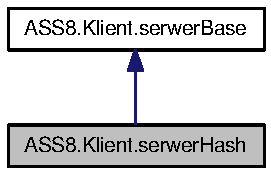
\includegraphics[width=166pt]{dd/dc1/a00212}
\end{center}
\end{figure}
\subsection*{Metody publiczne}
\begin{CompactItemize}
\item 
\hyperlink{a00024_79c7996d2e3af0a5ccceed0a8571f365}{serwerHash} ()
\item 
\hyperlink{a00024_c5d6f7f180298714d66df1b3651de900}{serwerHash} (int o, int op, string h)
\end{CompactItemize}
\subsection*{Właściwości}
\begin{CompactItemize}
\item 
string \hyperlink{a00024_7a7a7837aebfd93a49cc82322210f287}{hash}\hspace{0.3cm}{\tt  \mbox{[}get, set\mbox{]}}
\end{CompactItemize}
\subsection*{Atrybuty prywatne}
\begin{CompactItemize}
\item 
string \hyperlink{a00024_e3111f0da2c2e6180ae82949844b5111}{pHash}
\end{CompactItemize}


\subsection{Opis szczegółowy}
Klasa zawiera dane do serializacji odpowiedzi serwera na zapytanie o hash pliku. 



Definicja w linii 476 pliku XmlRequestsClass.cs.

\subsection{Dokumentacja konstruktora i destruktora}
\hypertarget{a00024_79c7996d2e3af0a5ccceed0a8571f365}{
\index{ASS8::Klient::serwerHash@{ASS8::Klient::serwerHash}!serwerHash@{serwerHash}}
\index{serwerHash@{serwerHash}!ASS8::Klient::serwerHash@{ASS8::Klient::serwerHash}}
\subsubsection[{serwerHash}]{\setlength{\rightskip}{0pt plus 5cm}ASS8.Klient.serwerHash.serwerHash ()}}
\label{dc/de2/a00024_79c7996d2e3af0a5ccceed0a8571f365}




Definicja w linii 479 pliku XmlRequestsClass.cs.\hypertarget{a00024_c5d6f7f180298714d66df1b3651de900}{
\index{ASS8::Klient::serwerHash@{ASS8::Klient::serwerHash}!serwerHash@{serwerHash}}
\index{serwerHash@{serwerHash}!ASS8::Klient::serwerHash@{ASS8::Klient::serwerHash}}
\subsubsection[{serwerHash}]{\setlength{\rightskip}{0pt plus 5cm}ASS8.Klient.serwerHash.serwerHash (int {\em o}, \/  int {\em op}, \/  string {\em h})}}
\label{dc/de2/a00024_c5d6f7f180298714d66df1b3651de900}




Definicja w linii 480 pliku XmlRequestsClass.cs.

\subsection{Dokumentacja atrybutów składowych}
\hypertarget{a00024_e3111f0da2c2e6180ae82949844b5111}{
\index{ASS8::Klient::serwerHash@{ASS8::Klient::serwerHash}!pHash@{pHash}}
\index{pHash@{pHash}!ASS8::Klient::serwerHash@{ASS8::Klient::serwerHash}}
\subsubsection[{pHash}]{\setlength{\rightskip}{0pt plus 5cm}string {\bf ASS8.Klient.serwerHash.pHash}\hspace{0.3cm}{\tt  \mbox{[}private\mbox{]}}}}
\label{dc/de2/a00024_e3111f0da2c2e6180ae82949844b5111}




Definicja w linii 478 pliku XmlRequestsClass.cs.

\subsection{Dokumentacja właściwości}
\hypertarget{a00024_7a7a7837aebfd93a49cc82322210f287}{
\index{ASS8::Klient::serwerHash@{ASS8::Klient::serwerHash}!hash@{hash}}
\index{hash@{hash}!ASS8::Klient::serwerHash@{ASS8::Klient::serwerHash}}
\subsubsection[{hash}]{\setlength{\rightskip}{0pt plus 5cm}string ASS8.Klient.serwerHash.hash\hspace{0.3cm}{\tt  \mbox{[}get, set\mbox{]}}}}
\label{dc/de2/a00024_7a7a7837aebfd93a49cc82322210f287}




Definicja w linii 487 pliku XmlRequestsClass.cs.

Dokumentacja dla tej klasy została wygenerowana z pliku:\begin{CompactItemize}
\item 
\hyperlink{a00055}{XmlRequestsClass.cs}\end{CompactItemize}
